\chapter{Cotas inferiores}

Retomamos el problema de admisión a universidades igual que como se plantea en el capíitulo 4, a cada universidad se le agrega la restricción de que necesita un número mínimo de alumnos asignados que necesitan para abrir. En particular se le agregan las siguientes tres ecuaciónes al problema:

\begin{enumerate}
\item \begin{equation} y_{j}= 
\begin{cases}
1 & \qquad \text{si la universidad $j$ abre.} \\
0 &\qquad\text{en otro caso.} \\ 
\end{cases} \end{equation} 
\item \begin{equation} \label{r6}
x_{i,j} \leq y_j \ \text{ para toda $i=1,2,\ldots,n$ y para toda $j=1,2,\ldots,m$.}
\end{equation}
Los solicitantes únicamente pueden asistir a universidades abiertas.
\item \begin{equation} \label{r4}
\sum_{i=1}^{n} x_{i,j} \geq\ m_j\times y_j 
\end{equation}
Cada universidad necesita admitir a una cantidad considerable de alumnos para abrir.
\end{enumerate}

Una pregunta inicial que surge es si todos los resultados obtenidos para el problema sin cotas inferiores o comunes se siguen cumpliendo, una vez que agregamos las cotas inferiores ¿el emparejamiento estable siempre existe? ¿De existir este es óptimo? ¿Se obtiene con facilidad? Para comenzar es posible mostrar que el emparejamiento estable no siempre existe.

\begin{eje}
\cite{Todo}\\
Supongamos que tenemos dos universidades $A$ y $B$, $A$ solo puede admitir a dos alumnos y necesita admitir a dos alumnos para entrar y $B$ solo puede admitir a un alumno y necesita a un alumno para abrir. Además, contamos con dos solicitantes $\alpha$ y $\beta$, la matriz de preferencias del problema está dada por 
$$\begin{pmatrix}
& A & B \\
\alpha & 1,1 & 2,1 \\
\beta & 2,2 & 1,2 \\ 
\end{pmatrix}.$$
Lo primero que notamos es que $A$ o $B$ tienen que estar cerradas porque la suma de las cotas inferiores es tres y solo contamos con dos estudiantes. Si $A$ cierra entonces tenemos dos emparejamientos posibles, en el primero $\alpha$ es admitido en $B$ y no es estable porque $\alpha$ prefiere estar en $A$, $\beta$ prefiere estar en $A$ a no estar en ningún lado y $A$ prefiere tener a los dos estudiantes que cerrar . 
\begin{figure}[H]\centering

\begin{tikzpicture}[ scale=0.8]
\tikzset{vertex/.style = {shape=circle,draw,minimum size=1.5em}}
\tikzset{edge/.style = {->,> = latex}}
\filldraw[color=blue!60, fill=blue!5, very thick](0,3) ellipse (.8 and 1.5);
\filldraw[color=green!60, fill=green!5, very thick](4,3) ellipse (.8 and 1.5);


% vertices
% 


\node[vertex] (a) at (0,4) {$\alpha$};
\node[vertex] (b) at (0,2) {$\beta$};


\node[vertex] (e) at (4,4) {$A$};
\node[vertex] (f) at (4,2) {$B$};


\node (i) at (0,5) {Solicitantes};
\node (j) at (4,5) {Universidades};

\path[-stealth] (a) edge (f);
%\path[-stealth] (b) edge (g);

\draw (4,4) node[cross=8pt,red] {};


%\draw (0.2,8)--(3.8,8);



\end{tikzpicture}

\caption{Primer caso.}
\end{figure}
En el segundo caso $\beta$ es admitido en $B$ y este emparejamiento no es estable porque $B$ prefiere tener a $\alpha$ que a $\beta$ y $\alpha$ prefiere estudiar que no estudiar. 
\begin{figure}[H]\centering

\begin{tikzpicture}[ scale=0.8]
\tikzset{vertex/.style = {shape=circle,draw,minimum size=1.5em}}
\tikzset{edge/.style = {->,> = latex}}
\filldraw[color=blue!60, fill=blue!5, very thick](0,3) ellipse (.8 and 1.5);
\filldraw[color=green!60, fill=green!5, very thick](4,3) ellipse (.8 and 1.5);


% vertices
% 


\node[vertex] (a) at (0,4) {$\alpha$};
\node[vertex] (b) at (0,2) {$\beta$};


\node[vertex] (e) at (4,4) {$A$};
\node[vertex] (f) at (4,2) {$B$};


\node (i) at (0,5) {Solicitantes};
\node (j) at (4,5) {Universidades};

\path[-stealth] (b) edge (f);
%\path[-stealth] (b) edge (g);

\draw (4,4) node[cross=8pt,red] {};


%\draw (0.2,8)--(3.8,8);



\end{tikzpicture}

\caption{Segundo caso.}
\end{figure}


Si $B$ cierra entonces solo tenemos un emparejamiento posible en el que $\alpha$ y $\beta$ son admitidos en $A$, este no es estable porque $B$ prefiere tener a $\beta$ que cerrar y $\beta$ prefiere estar en $A$ que en $B$.

\begin{figure}[H]\centering

\begin{tikzpicture}[ scale=0.8]
\tikzset{vertex/.style = {shape=circle,draw,minimum size=1.5em}}
\tikzset{edge/.style = {->,> = latex}}
\filldraw[color=blue!60, fill=blue!5, very thick](0,3) ellipse (.8 and 1.5);
\filldraw[color=green!60, fill=green!5, very thick](4,3) ellipse (.8 and 1.5);


% vertices
% 


\node[vertex] (a) at (0,4) {$\alpha$};
\node[vertex] (b) at (0,2) {$\beta$};


\node[vertex] (e) at (4,4) {$A$};
\node[vertex] (f) at (4,2) {$B$};


\node (i) at (0,5) {Solicitantes};
\node (j) at (4,5) {Universidades};

\path[-stealth] (a) edge (e);
\path[-stealth] (b) edge (e);

\draw (4,2) node[cross=8pt,red] {};


%\draw (0.2,8)--(3.8,8);



\end{tikzpicture}

\caption{Tercer caso.}
\end{figure}

\fin
\end{eje}

A partir de este ejemplo queda claro que si extendemos el problema agregando cotas inferiores perdemos la garantía de existencia de un emparejamiento estable en nuestro problema. Es posible además construir un algoritmo a partir del algoritmo de Gale Shapley para admisión a universidades que converja en caso de que exista a un emparejamiento estable o que saque como resultado si no existe un emparejamiento estable para este problema, el algoritmo esta dado por el siguiente código. Antes de mostrarlo vale la pena recordar que si tienes $m$ universidades entonces existen $2^{m}-1$ (corolario \ref{card3}) posibles combinaciones de qué universidades mantienen abiertas y cuales cierran. 
%\begin{lstlisting}[style=R, escapeinside={(*}{*)},caption={Algoritmo de Gale Shapley para admisión a universidades con cotas inferiores}, captionpos=b, label=c3]
%Input : Una matriz de preferencias para (*$n$*) solicitantes y (*$m$*) universidades, un vector (*$M$*) en donde la entrada (*$j$*) representa la cota superior de la universidad (*$j$*) y un vector (*$N$*) en donde la entrada (*$j$*) representa la cota inferior de la universidad (*$j$*).
%Output: Un emparejamiento o mensaje. 
%repeat{ #Hasta encontrar un emparejamiento estable factible.
%Se selecciona una de las (*$2^{m}-1$*) combinaciones, se escoge primero las opciones que cierren menos universidades de las todavía no escogidas. 
%Cada universidad abierta invita a los primeros (*$j_i$*) solicitantes en su lista a estudiar ahí. Cada alumno que recibe más de una solicitud acepta las más alta en su lista y rechaza el resto. 
%repeat{ #hasta que cada universidad abierta este llena o cuando todos los estudiantes sean admitidos en una universidad.
%Las universidades que no alcanzaron su cota superior invitan a los siguientes alumnos de su lista de acuerdo con cuantos lugares tienen.
%Cada solicitante que recibe una solicitud acepta la más alta en su alta entre su actual universidad y las que lo invitaron. 
%El alumno rechaza el resto de las invitaciones.
%}
%Si la asignación obtenida es factible, el algoritmo acaba y saca como output el emparejamiento. 
%}
%Si el algoritmo trato todas las combinaciones y no encontró un emparejamiento estable factible entonces saca un mensaje diciendo que este no existe.
%\end{lstlisting}
\vspace{1 cm}

\IncMargin{1em}
\begin{Algoritmo}[H]
%\SetKwData{Left}{left}\SetKwData{This}{this}\SetKwData{Up}{up}
%\SetKwFunction{Union}{Union}\SetKwFunction{FindCompress}{FindCompress}
\SetKwInOut{Input}{input}\SetKwInOut{Output}{output}

\Input{Una matriz de preferencias para $n$ solicitantes y $m$ universidades, un vector $M$ en donde la entrada $j$ representa la cota superior de la universidad $j$ y un vector $N$ en donde la entrada $j$ representa la cota inferior de la universidad $j$.}
\Output{Un emparejamiento o un mensaje.}
\BlankLine
\Repeat{Hasta encontrar un emparejamiento estable factible o hasta tratar todas las combinaciones}{
	\emph{Se selecciona una de las $2^{m}-1$ combinaciones, se escoge primero las opciones que cierren menos universidades de las todavía no escogidas\;}
	\emph{Se le aplica el algoritmo de Gale Shapley para admisión de universidades a la combinación de universidades abiertas y se obtiene una asiignación\;}
	\emph{Si la asignación obtenida es factible, el algoritmo acaba y saca como output el emparejamiento\;}
	}
	\emph{Si el algoritmo trato todas las combinaciones y no encontró un emparejamiento estable factible entonces saca un mensaje diciendo que este no existe\;}
\caption{Gale Shapley  para admisión a universidades con cotas inferiores.}
\end{Algoritmo}
\DecMargin{1em}

\begin{cor}
Dada una matriz de preferencias arbitraria, un vector de cotas superiores arbitrario y un vector de cotas inferiores arbitrario, el algoritmo de Gale Shapley para admisión a universidades con cotas inferiores converge.
\end{cor}
\begin{proof}
Supongamos que existe una combinación de universidades abiertas que cuenta con una asignación estable y el algoritmo no la encuentra. Esto es, existe una combinación de universidades en las que el emparejamiento estable producido por Gale Shapley no es factible, pero en la que si existe un emparejamiento estable factible, lo cual es una contradicción al teorema \ref{rural} porque todos los emparejamientos estables asignan exactamente el mismo número de personas a cada universidad y por lo tanto si el emparejamiento encontrado por el algoritmo no es factible eso implicaría que todas las asignaciones estables no son factibles. \\
Cómo se escoge las opciones que cierren menos universidades de las todavía no escogidas podemos garantizar que de encontrar un emparejamiento estable factible este no tiene una universidad bloqueadora. 
Además, porque el algoritmo trata todas las combinaciones y porque el corolario \ref{gsu} nos garantiza que dada una combinación de universidades abiertas el algoritmo siempre encuentra un emparejamiento estable, entonces podemos concluir que de existir un emparejamiento estable factible el algoritmo de Gale Shapley para admisión a universidades con cotas inferiores lo va a encontrar y por lo tanto el algoritmo converge a lo deseado. 
\end{proof}

Este algoritmo a diferencia de los anteriores en que tiene la enorme desventaja de que no es muy eficiente, si el número de universidades es muy grande el algoritmo podría no acabar porque el poder de computo necesario para correrlo es exponencial respecto al número de universidades, esto queda fundamentado por el siguiente resultado.
\begin{cor}
La complejidad del algoritmo de Gale Shapley para admisión a universidades con cotas inferiores es del orden de $2^{m}\cdot m^2$, donde $m$ es el número de universidades.
\end{cor}
\begin{proof}
En el peor escenario no existe una asignación estable factible para el problema, en este caso se realiza $2^{m}-1$ veces el algoritmo de Gale Shapley, que por la observación \ref{complejidad1} tiene como complejidad $m^2$. Por lo tanto, el número máximo de pasos que tiene el algoritmo es aproximadamente $(2^{m}-1)\cdot m^2=2^{m}\cdot m^2-m^2$ y podemos concluir que la complejidad del algoritmo es del orden de $2^{m}\cdot m^2$.
\end{proof}

A continuación mostramos un ejemplo de cómo funciona el algoritmo para dejarlo más claro. 
\begin{eje}
\cite{Todo}\\
Supongamos que tenemos dos universidades $A$ y $B$, $A$ tiene como cota inferior a dos estudiantes y solo puede admitir a dos solicitantes, $B$ necesita a tres estudiantes para abrir y tiene como cota superior a tres alumnos. Además, a esto contamos con tres solicitantes $\alpha$, $\beta$ y $\gamma$, la matriz de preferencias para este problema es 
$$\begin{pmatrix}
& A & B \\
\alpha & 1,1 & ,1 \\
\beta & 1,2 & 2,1 \\ 
\gamma & , & 1,2 \\ 
\end{pmatrix}$$
En el primer paso del algoritmo las dos universidades se mantienen abiertas, $\alpha$ aplica a $A$, $\beta$ aplica a $A$ y $\gamma$ aplica a $B$. $A$ y $B$ aceptan a los tres alumnos llegando a una asignación estable pero no factible. 
\begin{figure}[H]\centering

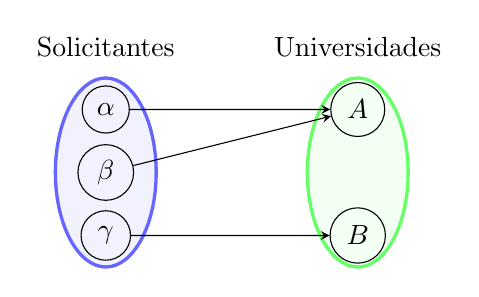
\begin{tikzpicture}[ scale=0.8]
\tikzset{vertex/.style = {shape=circle,draw,minimum size=1.5em}}
\tikzset{edge/.style = {->,> = latex}}
\filldraw[color=blue!60, fill=blue!5, very thick](0,3) ellipse (.8 and 1.5);
\filldraw[color=green!60, fill=green!5, very thick](4,3) ellipse (.8 and 1.5);


% vertices
% 


\node[vertex] (a) at (0,4) {$\alpha$};
\node[vertex] (b) at (0,3) {$\beta$};
\node[vertex] (c) at (0,2) {$\gamma$};


\node[vertex] (e) at (4,4) {$A$};
\node[vertex] (f) at (4,2) {$B$};


\node (i) at (0,5) {Solicitantes};
\node (j) at (4,5) {Universidades};

\path[-stealth] (a) edge (e);
\path[-stealth] (b) edge (e);
\path[-stealth] (c) edge (f);

%\draw (4,2) node[cross=8pt,red] {};


%\draw (0.2,8)--(3.8,8);



\end{tikzpicture}

\caption{Primera iteración.}
\end{figure}

En el segundo paso del algoritmo $A$ cierra y $B$ se mantiene abierto. $\alpha$ no aplica a ninguna universidad, $\beta$ aplica a $B$ y $\gamma$ aplica a $B$. $B$ acepta a los dos alumnos llegando a un emparejamiento estable pero no factible.
\begin{figure}[H]\centering

\begin{tikzpicture}[ scale=0.8]
\tikzset{vertex/.style = {shape=circle,draw,minimum size=1.5em}}
\tikzset{edge/.style = {->,> = latex}}
\filldraw[color=blue!60, fill=blue!5, very thick](0,3) ellipse (.8 and 1.5);
\filldraw[color=green!60, fill=green!5, very thick](4,3) ellipse (.8 and 1.5);


% vertices
% 


\node[vertex] (a) at (0,4) {$\alpha$};
\node[vertex] (b) at (0,3) {$\beta$};
\node[vertex] (c) at (0,2) {$\gamma$};


\node[vertex] (e) at (4,4) {$A$};
\node[vertex] (f) at (4,2) {$B$};


\node (i) at (0,5) {Solicitantes};
\node (j) at (4,5) {Universidades};

%\path[-stealth] (a) edge (e);
\path[-stealth] (b) edge (f);
\path[-stealth] (c) edge (f);

\draw (4,4) node[cross=8pt,red] {};


%\draw (0.2,8)--(3.8,8);



\end{tikzpicture}

\caption{Segunda iteración.}
\end{figure}

En el tercer paso del algoritmo $B$ cierra y $A$ se mantiene abierto. $\gamma$ no aplica a ninguna universidad, $\alpha$ aplica a $A$ y $\alpha$ aplica a $A$. $A$ acepta a los dos alumnos llegando a un emparejamiento estable factible. Después de 3 pasos en el
algoritmo, encontramos un emparejamiento estable factible, es decir, el algoritmo convergió.
\begin{figure}[H]\centering

\begin{tikzpicture}[ scale=0.8]
\tikzset{vertex/.style = {shape=circle,draw,minimum size=1.5em}}
\tikzset{edge/.style = {->,> = latex}}
\filldraw[color=blue!60, fill=blue!5, very thick](0,3) ellipse (.8 and 1.5);
\filldraw[color=green!60, fill=green!5, very thick](4,3) ellipse (.8 and 1.5);


% vertices
% 


\node[vertex] (a) at (0,4) {$\alpha$};
\node[vertex] (b) at (0,3) {$\beta$};
\node[vertex] (c) at (0,2) {$\gamma$};


\node[vertex] (e) at (4,4) {$A$};
\node[vertex] (f) at (4,2) {$B$};


\node (i) at (0,5) {Solicitantes};
\node (j) at (4,5) {Universidades};

\path[-stealth] (a) edge (e);
\path[-stealth] (b) edge (e);
%\path[-stealth] (c) edge (f);

\draw (4,2) node[cross=8pt,red] {};


%\draw (0.2,8)--(3.8,8);



\end{tikzpicture}

\caption{Tercera iteración.}
\end{figure}


\fin
\end{eje}


Al igual que en las secciones anteriores el algoritmo puede ser modificado para que sea optimo para las universidades, los resultados de convergencia y de complejidad son analogos a los mostrados.
Además a esto, \cite{Todo} propone una heuristica para resolver este problema de forma rapida. En general hay que tener cuidado al usarla porque el algoritmo ignora la existencia de universidades bloqueadoras y podria no llegar a una solución a pesar de que para ese problema en particular si exista una asignación estable.
\\
\IncMargin{1em}
\begin{Algoritmo}[H]
%\SetKwData{Left}{left}\SetKwData{This}{this}\SetKwData{Up}{up}
%\SetKwFunction{Union}{Union}\SetKwFunction{FindCompress}{FindCompress}
\SetKwInOut{Input}{input}\SetKwInOut{Output}{output}
\Input{Una matriz de preferencias para $n$ solicitantes y $m$ universidades, un vector $M$ en donde la entrada $j$ representa la cota superior de la universidad $j$ y un vector $N$ en donde la entrada $j$ representa la cota inferior de la universidad $j$.}
\Output{Un emparejamiento o un mensaje.}
\BlankLine
\emph{$U$ $\gets$ un vector de tamaño $m$ con los nombres de todas las universidades\;}
\Repeat{Hasta encontrar un emparejamiento estable factible o mientras $U$ sea no vacio}{
	\emph{Se aplica el algoritmo de Gale Shapley para admisión a universidades considerando que las escuelas que aparecen en $U$ estan abiertas y las que no estan cerradas obteniendo un emparejamiento $M$\;}
	\eIf{$M$ es factible}{
		El algoritmo acaba y saca como output el emparejamiento\;
		}
		{
		\emph{Sea $A$ la universidad con el cociente entre el número asignado de estudiantes y su cota inferior mínimo \;}
		\emph{$U$ $\gets$ $U \setminus A$ (Al vector $U$ le quitamos la universidad $A$) \;} 
		}
}
\emph{Si $U$ esta vacio, saca un mensaje diciendo que no se encontro el emparejamiento\;}
\caption{Heuristica  para admisión a universidades con cotas inferiores.}
\end{Algoritmo}
\DecMargin{1em}

%no siempre converge
%heuristicas
%es np completo

